\documentclass[border=10pt]{standalone}
\usepackage[utf8]{inputenc}
\usepackage[T1]{fontenc}
\usepackage{tikz}
\usetikzlibrary{shapes.geometric, arrows.meta, positioning, fit, backgrounds, shadows}

\begin{document}

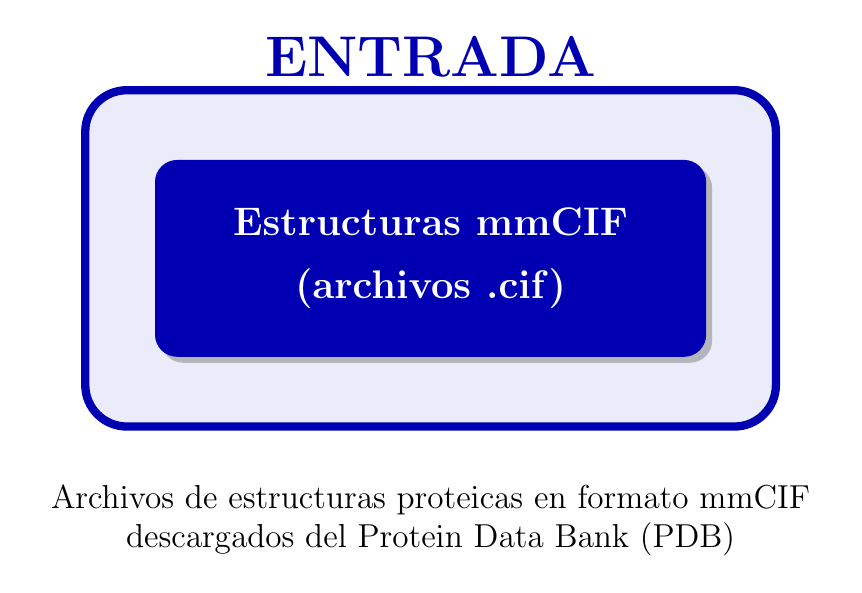
\begin{tikzpicture}[
        % Estilo para entrada
        inputbox/.style={
                rectangle,
                rounded corners=8pt,
                minimum height=2.5cm,
                minimum width=7cm,
                text centered,
                text width=6cm,
                font=\bfseries\Large,
                text=white,
                fill=blue!70!black,
                drop shadow
            },
        % Grupo contenedor
        groupbox/.style={
                rectangle,
                rounded corners=15pt,
                draw=blue!70!black,
                line width=3pt,
                fill=blue!70!black!8,
                inner sep=25pt
            }
    ]

    % ENTRADA
    \node[inputbox] (pdb) {Estructuras mmCIF\\[5pt](archivos .cif)};

    % Grupo de entrada
    \begin{scope}[on background layer]
        \node[groupbox, fit=(pdb), label={[font=\bfseries\huge, text=blue!70!black]above:ENTRADA}] (entrada) {};
    \end{scope}

    % Descripción
    \node[below=1.5cm of pdb, text width=10cm, align=center, font=\large] {
        Archivos de estructuras proteicas en formato mmCIF\\
        descargados del Protein Data Bank (PDB)
    };

\end{tikzpicture}

\end{document}
